\documentclass[aspectratio=169]{beamer}

\usepackage{tikzlings}

\setbeamertemplate{navigation symbols}{}
\setbeamertemplate{background canvas}{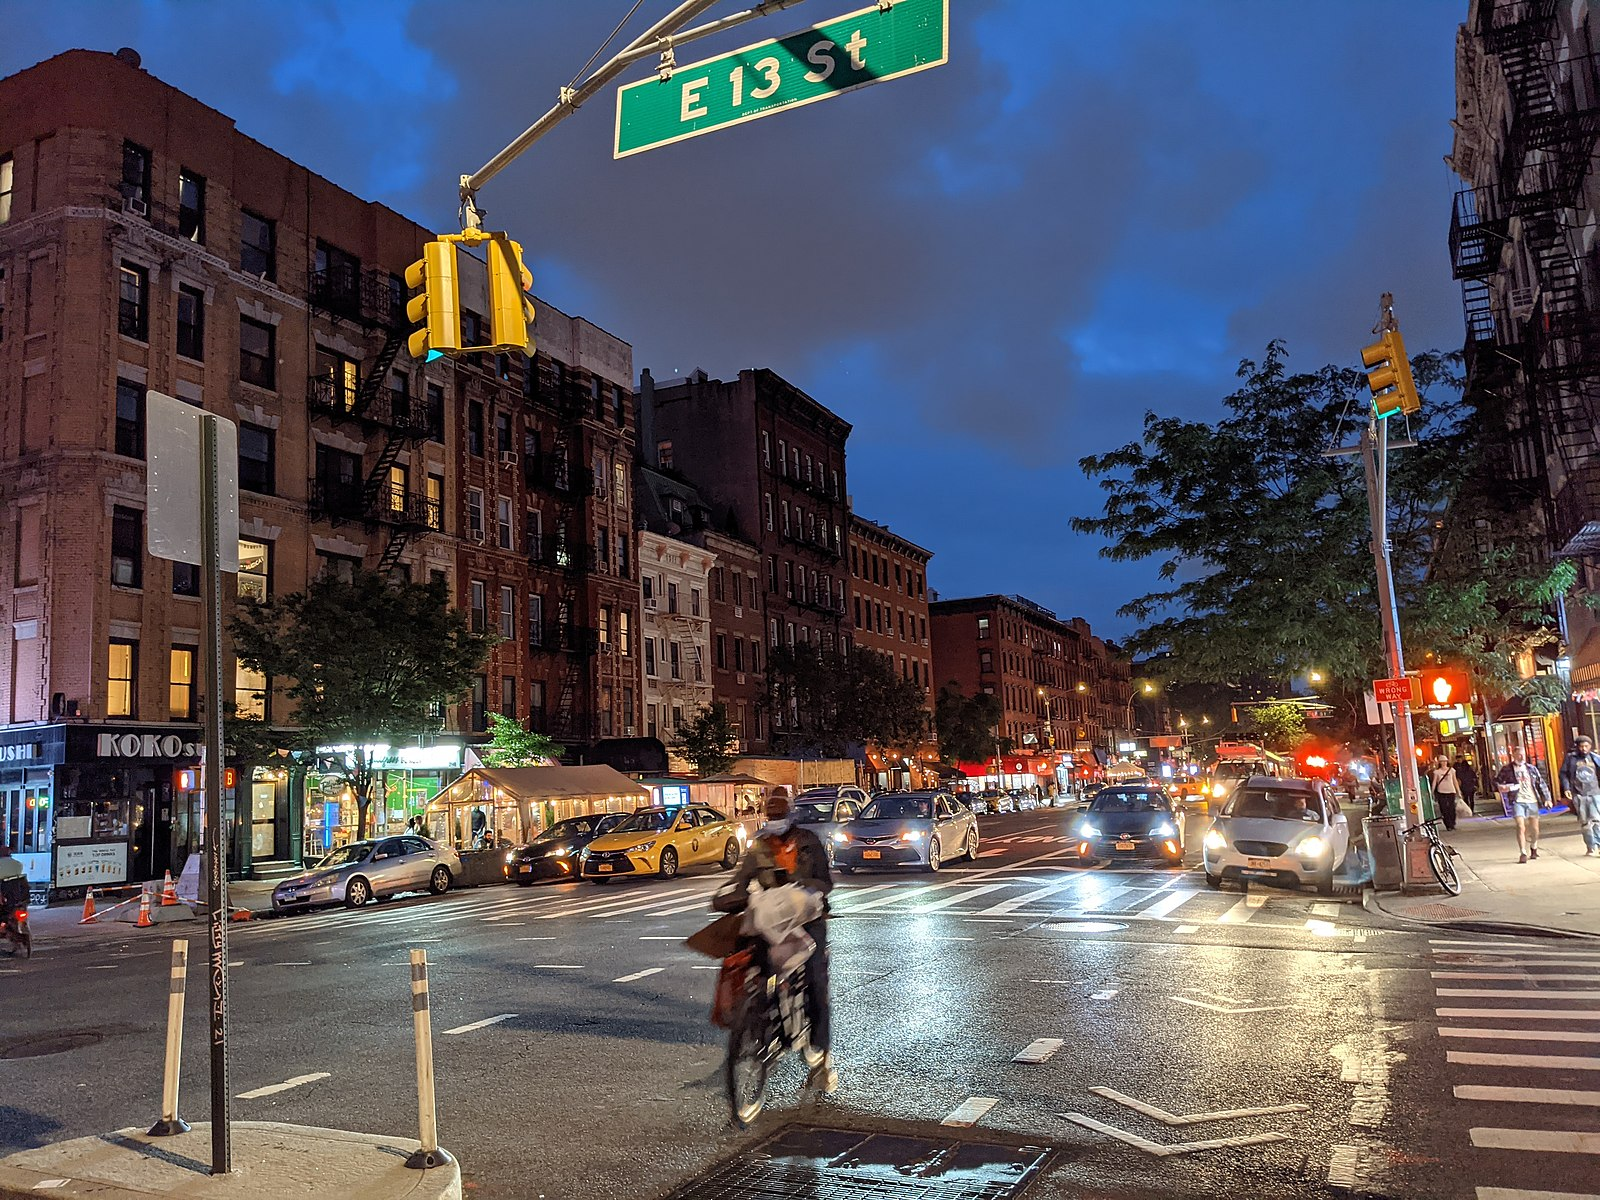
\includegraphics[width=\paperwidth]{Nightfall_on_13th_Street_(51246144554).jpg}}

% trick taken from https://topanswers.xyz/tex?q=1989
\tikzset{
    use page relative coordinates/.style={
        shift={(current page.south west)},
        x={(current page.south east)},
        y={(current page.north west)}
    },
}
\definecolor{sloth}{RGB}{137,126,88}

\begin{document}
	
\begin{frame}
  \begin{tikzpicture}[remember picture, overlay,use page relative coordinates]

    % some movement
    %\fill[red] (\thepage/600,1-\thepage/600) circle [radius=0.2cm];
    
    % showing a couple of example coordinates
    %\node[anchor=south west] at (0,0) {(0,0)};
%    \node[anchor=south east] at (1,0) {(1,0)};
%    \node[anchor=north west] at (0,1) {(0,1)};
%    \node[anchor=north east] at (1,1) {(1,1)};
%    
    % credit for background image
    \node[white,text width=.7\paperwidth,font=\tiny,align=center] at ([yshift=0.35cm]current page.south) {Image source: \url{xxx}};  
 
  \begin{scope}[x=1cm,y=1cm,shift={(-1cm,0.98\textheight)}]  
 \foreach \x in %{1} {
 {1,0.995,...,0}{%

	%Body of the sloth
	\fill<+>[sloth] 
	(7.177, -0.504) .. controls ( 7.170, -1.471) and (7.144, -2.099) ..
	(7.566, -2.687) .. controls ( 8.103, -3.436) and (9.188, -3.187) ..
	(9.754, -2.806) .. controls (10.545, -2.330) and (9.871, -1.241) ..
	(9.871, -1.241) .. controls ( 9.655, -1.440) and (9.853-\x*0.5, -0.542-\x) ..
	(9.684-\x*0.7, -0.163-\x*0.5) .. controls ( 9.495-\x*0.7,  0.262-\x*0.5) and (9.227-\x*0.8, -0.049-\x*0.55) ..
	(9.219-\x*0.7, -0.205-\x*0.55) .. controls ( 9.577-\x*0.36, -1.771) and (8.413, -2.548) ..
	(8.395, -0.901) -- 
	(8.069, -0.950) .. controls ( 8.073, -1.333) and (8.130, -1.661) ..
	(8.031, -1.697) .. controls ( 7.539, -1.787) and (7.677, -0.756) .. 
	(7.577, -0.386) .. controls ( 7.516, -0.162) and (7.182, -0.365) .. 
	(7.177, -0.504) -- cycle;

	% Head
	\node<.>[rotate=-55+\x*25] at (10.3, -1.7) {
\includegraphics[width=1.6cm]{sloth_head}};	
	
	% front paw	
	\fill<.>[sloth!40!black,rotate around={10+\x*22:(9.6,-2.5)}] (9.84, 0.02-\x*0.33) ellipse (0.06 and 0.18);
	\fill<.>[sloth!40!black,rotate around={0+\x*22:(9.6,-2.5)}] (9.55+\x*0.05, 0.05-\x*0.35) ellipse (0.06 and 0.18);
	\fill<.>[sloth!40!black,rotate around={20+\x*22:(9.6,-2.5)}] (10.12-\x*0.05, -0.08-\x*0.3) ellipse (0.06 and 0.18);		
		
}

% back paw
\begin{scope}[rotate=10]
\fill[sloth!40!black,rotate around={0:(7.21, -1.57)}] (7.21, -1.57) ellipse (0.06 and 0.18);
\fill[sloth!40!black,rotate around={-15:(7.37, -1.6)}] (7.37, -1.6) ellipse (0.06 and 0.18);
\fill[sloth!40!black,rotate around={10:(7.05, -1.6)}] (7.05, -1.6) ellipse (0.06 and 0.18);	
\end{scope}		   
 \end{scope}   
  \end{tikzpicture}
 % \pause[20]
\end{frame}	

	
\end{document}
